%---------------------------------------------------
% Nombre: capitulo2.tex  
% 
% Texto del cap�tulo 2
%---------------------------------------------------

\chapter{Experimento de datos}
\label{dos}

En este cap�tulo, realizaremos las consultas sobre la base de datos para ello, nos pondremos en lugar de un hipot�tico cient�fico de datos para obtener informaci�n acerca de las quejas de los usuarios.

\section{Carga de datos}

Lo primero que hacemos es cargar los datos en PIG. Para ello, primero debemos de tener los datos en el HDFS.

{\small
\begin{verbatim}
hdfs dfs -put ConsumerComplaints.csv /user/impala/CD_DNI/input
hdfs dfs -ls /user/impala/CD_DNI/input
\end{verbatim}
}
	 
Una vez tenemos los datos en el HDFS, los cargamos en una estructura de PIG en funci�n del esquema.


{\small
\begin{verbatim}
	complaint = load
  	'/user/impala/CD_DNI/input/ConsumerComplaints.csv'
 	 using PigStorage(',') AS (DateReceived :chararray,
 	 ProductName:chararray, SubProduct:chararray,Issue:chararray,
 	 SubIssue:chararray,ConsumerComplaintNarrative:chararray, 
	 CompanyPublicResponse:chararray, Company:chararray,
	 StateName:chararray, ZipCode:chararray, Tags:chararray,
 	 ConsumerConsentProvided:chararray, SubmittedVia:chararray, 
	 DateSenttoCompany:chararray,CompanyResponsetoConsumer:chararray,
	 TimelyResponse:chararray, ConsumerDisputed:chararray,ComplaintID:chararray);
\end{verbatim}
}

\section{Proceso exploratorio}

Somos nuevos en la compa��a y se nos ha contratado para analizar si las quejas de los usuarios est�n siendo contestadas a tiempo o no y ver como mejorar este sector de la compa��a, por tanto la primera pregunta a resolver ser�a:

\textit{\textbf{�Cuales son los posibles valores del campo TimelyResponse?}}


Para ello, hay que ejecutar una selecci�n de aquellos que sean distintos.

{\small
\begin{verbatim}
distinct_timely_response = foreach complaint generate TimelyResponse;
result = distinct distinct_timely_response;
dump result;
\end{verbatim}
}

La salida de la consulta  podemos verla en la figura \ref{1}. 
\begin{figure}[H]
	\centering
		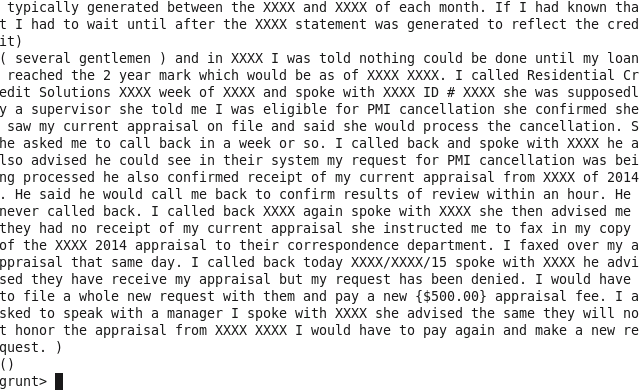
\includegraphics[scale=0.5]{./Capitulo2/imagenes/1.png}
		\caption{Salida de la consulta 1.}
	\label{1}
\end{figure}

Parece que no hemos tenido buenos resultados ya que a pesar de lo que podr�amos pensar hay muchos tipos de contenido en esta tabla en lugar de respuestas a la pregunta si se ha respondido en tiempo. Vamos a intentar obtener aquellos registros m�s comunes, es decir, que se repitan m�s de 100 veces a ver si as� localizamos la informaci�n buscada. Para ello, debemos responder a la pregunta:

\textit{\textbf{�Cuales son los valores m�s comunes del campo TimelyResponse?}}

Para esta consulta debemos hacer varias conjuntas:

{\small
\begin{verbatim}
grupo  = GROUP complaint by TimelyResponse;
cuenta = FOREACH grupo GENERATE group, 
	      COUNT(complaint.TimelyResponse) AS total;
filtro = FILTER cuenta BY total > 300; 
dump filtro;
\end{verbatim}
}

La salida de esta consulta est� en el gr�fico \ref{2}. En el podemos comprobar como si que hemos tenido efecto y tenemos ante nosotros las categor�as m�s usadas dentro de esta columna, lo que nos lleva a saber que la mayor�a de las quejas se cierran en tiempo, aunque hay otras que se cierran con ciertas caracter�sticas especiales como \textbf{Closed With Monetary Relief}. 
	
\begin{figure}[H]
	\centering
		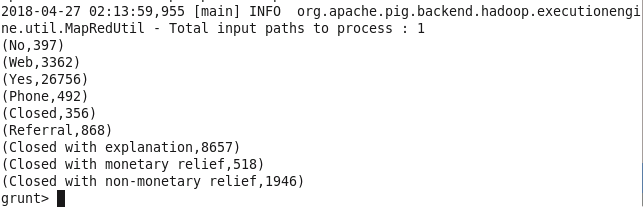
\includegraphics[scale=0.6]{./Capitulo2/imagenes/2.png}
		\caption{Salida de la consulta 2.}
	\label{2}
\end{figure}


Por �ltimo, localizado este �tem vamos a trazar un paralelismo entre los casos cerrados con \textbf{Closed With Monetary Relief} y las fechas de cierre, para tratar de localizar si hay m�s quejas en periodos como despu�s de navidad que buscan recibir el dinero de las compras de navidad y por tanto se generan quejas falsas. Para esta consulta:


{\small
\begin{verbatim}
	filter_complaint = FILTER complaint BY 
				TimelyResponse=='Closed with monetary relief';
	grupo_complaint = GROUP filter_complaint BY DateReceived;
	cuenta_fechas = FOREACH grupo_complaint 
				  GENERATE group,COUNT(filter_complaint.DateReceived) AS total;
	filtro_final = FILTER cuenta_fechas BY total > 3;
	ordenados = order filtro_final by total desc;
	dump ordenados;
\end{verbatim}
}


El resultado de esta consulta podemos verlo en la figura \ref{3}. Donde podemos concluir que no hay un patr�n claro y por tanto a priori podr�amos descartar los fraudes. 

\begin{figure}[H]
	\centering
		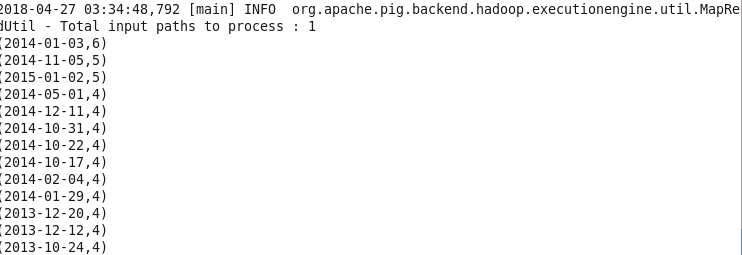
\includegraphics[scale=0.5]{./Capitulo2/imagenes/3.png}
		\caption{Salida de la consulta 3.}
	\label{3}
\end{figure}


\pagebreak
\clearpage
%---------------------------------------------------